
\chapter{Introduction} \label{chapter:introduction}
\section{Overview}

% Overview
% * applications need a map
% * methods have been evolving, fueled by new sensors. In particular RGB-D
%   RGB-D Sensors
%   * Specs of RGB-D sensors, create lots of data
%   * Mapping methods must be able to handle this data
%   Maps
%   * slam problem, we are concerned with mapping
%   * types of maps, we are concerned with rich types
%   * list of constraints: supported, computation, memory
%   * discussion of why mesh
% Goal
% * Create a system that can intelligently make decisions about sensor data
%   * Using tools already developed for mesh
%   * Computationally feasible
%   * Leverage information that we already know
% Contribution
% * Discussion of difference with "black box" methods

Many robotic applications, especially those that involve human-robot
interaction, often require a rich representation of the environment in order to
perform such behavior as path planning and obstacle avoidance. In general, a
rich representation, or map, is useful for providing situational awareness to an
autonomous agent. A map is also important for applications such as teleoperation
\cite{Kadous2006}.

In robotics, map building in an unknown environment is referred to as the
Simultaneous Localization and Mapping (SLAM) problem \cite{Thrun2002}. This
label describes the fact that a methodology which solves the SLAM problem must
simultaneously locate the robot in the environment as well as map the
environment. The focus of this work is the mapping aspect of the SLAM problem.
Fig. \ref{fig:goal} gives a visualization of the goal.

\begin{figure}[h]%[thpb]
\centering
  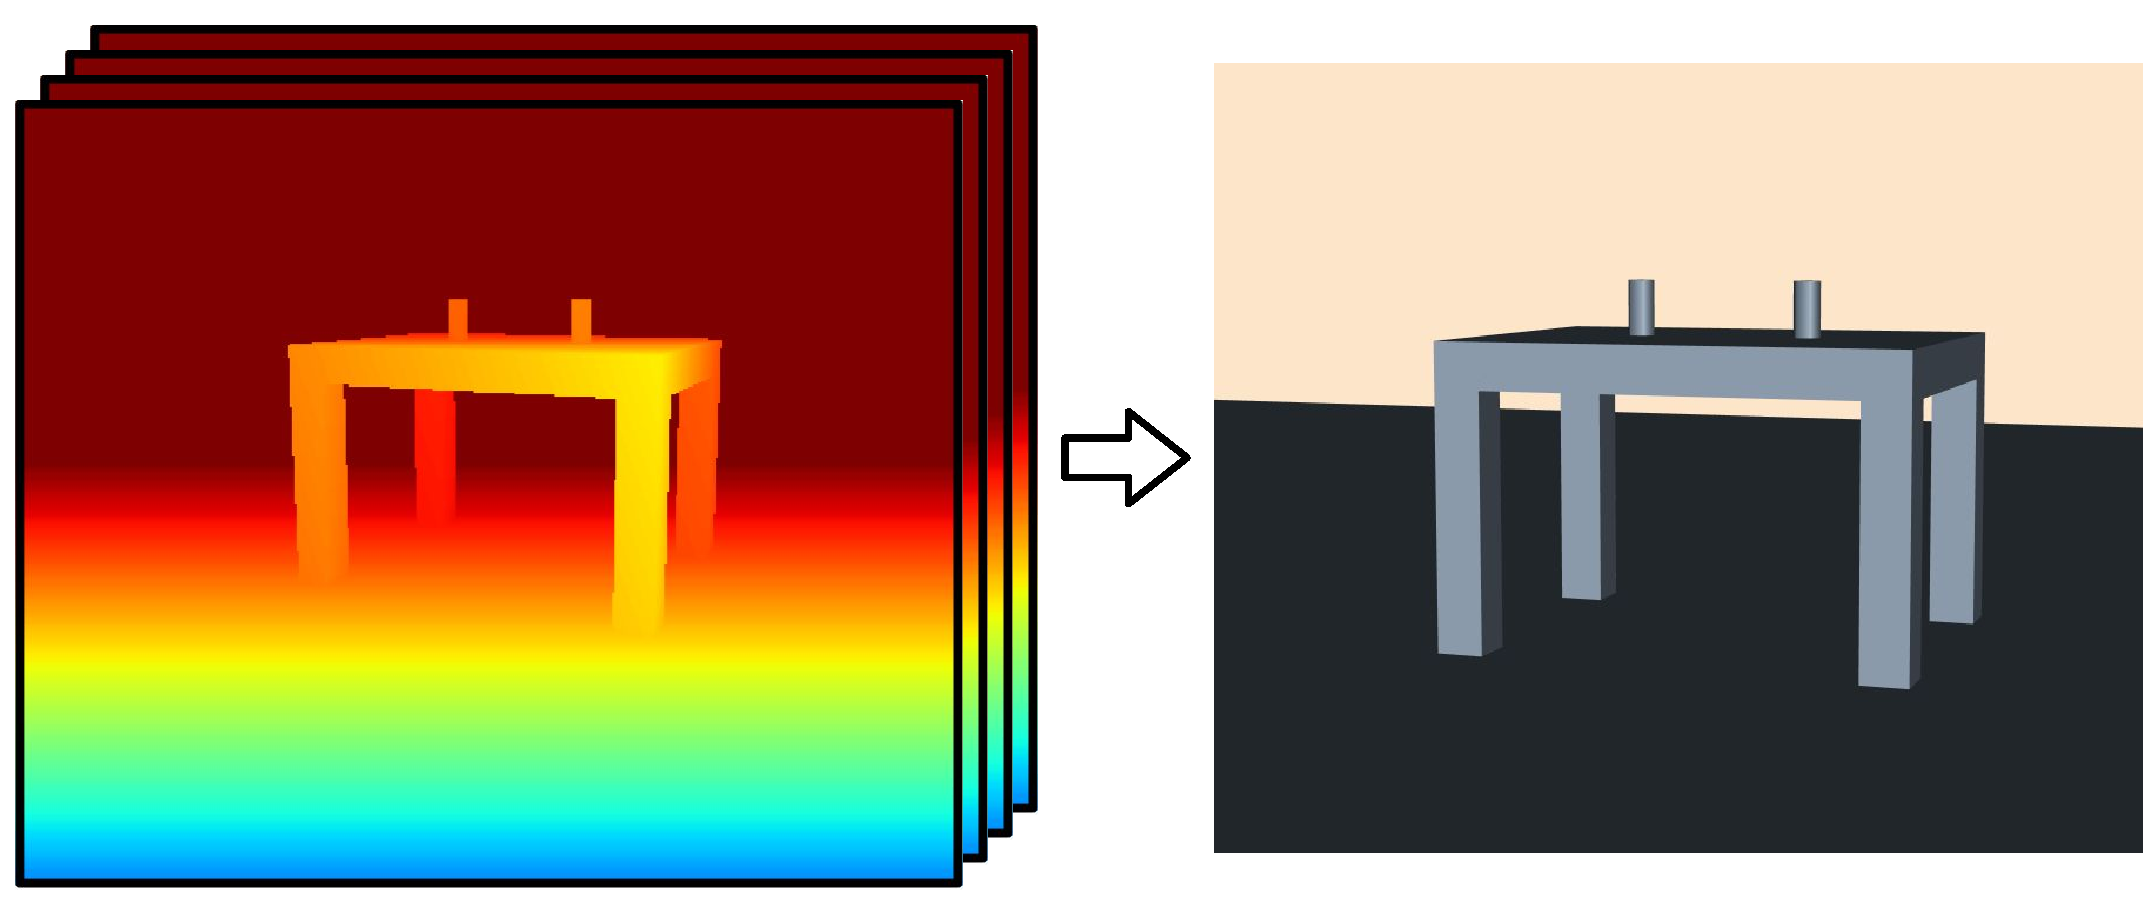
\includegraphics[width=.75\textwidth]{figures/intro_goal.pdf}
  \caption{Goal is to create a map from depth images.}
  \label{fig:goal}
\end{figure}

The methodology to build a map is a continuously evolving subject in the field
of robotics and computer graphics. Well known works of map building methods
began to be seen around 1987 \cite{Lorensen1987}. Since then, the methods and
the representations themselves have continued to evolve at an impressive rate.
Growth in this field of research has been fueled by continuous advances in
computing and sensing technologies. Over the years, sensors have continued to
generate measurements at higher rates, higher resolution, and lower cost. RGB-D
sensors are a new category of sensor that have recently gained extensive
popularity in the robotics community due to their affordability and ability to
generate a rich amount of data.

\subsection{RGB-D Sensors}

The popularity of RGB-D sensors began with the release and commercialization of
the Kinect\texttrademark ~ by Microsoft. The arrival of the Kinect brought with
it an inexpensive depth sensor that uses an active range system to generate a
depth map of a given environment \cite{freedman2012depth}. The Kinect and
similar sensors, have come to be called RGB-D sensors. This class of sensors
provide images which include both visual (RGB) and depth (D) values. Several
works have taken advantage of this sensor technology in scenarios such as
environmental mapping \cite{henry2012rgb}, 3D reconstruction
\cite{Newcombe2011a}, gesture recognition \cite{Xia2011}, and altitude control
of aerial vehicles \cite{Stowers2011}.

RGB-D sensors generally provide data at 30 frames per second and 640$\times$480
resolution. Consequently, methods that use RGB-D data must handle over 9 million
pixel values per second, if only using the depth information (D), and over 18
million if using both color (RGB) and depth (D). The amount of
data output from RGB-D sensors creates the need for mapping methods that are
computationally inexpensive and also influences the type of data structure used
to store the map.

\subsection{Maps}

There are different types of data structures that can define a map. All types
have both intrinsic characteristics that impact the algorithms that generate
them and constraints that must be considered for real-world applications. In
addition, we are concerned with rich representation types, in contrast to sparse
representation types \cite{Dissanayake2001}, because rich types have the most
use in applications such as human-robot interaction.

\begin{table}[h]
  \caption{Comparison of constraints for different map types.}
  \label{tab:rep}
  \begin{footnotesize}
  \begin{center}
    \begin{tabular}{|l|c|c|c|c|c|}
    \hline
    \multirow{2}{*}{}   & Supported & Computationally & Low Memory  \\
                        &           & Inexpensive     & Requirement \\\hline
    Point Clouds		    & x         & x               & -           \\
    Surfels             & -         & x               & x           \\
    Implicit Functions 	& x         & -               & -           \\
    Mesh	 	            & x         & x               & x           \\
    \hline
    \end{tabular}
  \end{center}
  \end{footnotesize}
\end{table}

When considering which type of map is best for real-world applications, we must
consider the constraints imposed by each type:

\begin{itemize}
  \item Supported - Is there software, tools, research, algorithms, etc., for
  this type of map?
  \item Computationally Inexpensive - Can the algorithms run quickly on low cost
  computers (rather than specialized hardware)?
  \item Low Memory Requirement - Can the algorithms run on hardware with
  a standard amount of RAM?
\end{itemize}

Table \ref{tab:rep} compares the constraints of common map types. We can see, in
general a mesh type map satisfies real-world constraints. Additionally, meshes
have been used extensively by the gaming and graphics communities, and so
benefits from an incredible amount of continued research and advances in
hardware such as Graphics Processing Units (GPUs).

\section{Goal}

The goal of this work is to develop a mapping algorithm that can gracefully
utilize the amount of data output from an RGB-D sensor. Additionally, the
algorithm will make use of software tools and hardware that have been developed
for mesh data structures. The algorithm will be able to make intelligent
decisions using the data it receives based on the knowledge it has been building
about the environment. The decisions will be driven by the leveraging the
difference between what the algorithm is actually seeing and what it expects to
see. The decisions will be generated using computationally inexpensive computer
vision methods.

\section{Contribution}

MABDI's contribution to the state-of-the-art in mesh based environmental mapping
is closing the loop of the algorithmic structure used by current methods. Fig.
\ref{fig:pipeline_cs} shows the structure of current methods. Data comes in from
the sensor, those measurements are used to create a mesh, and then that mesh is
appended to a global mesh. We can then compare the structure of current methods
to the structure used in MABDI, shown in Fig. \ref{fig:pipeline_mabdi}. Both
structures have the ``Create Mesh from Input'' component. The input to this
component is different for current methods and MABDI. Current methods input all
data from the sensor whereas MABDI only inputs data identified to be from the
unknown parts of the environment. The MABDI algorithm is able to identify this
data by leveraging the knowledge contained in the Global Mesh and intelligently
categorizing the incoming data. This categorization of the incoming data closes
the loop of the algorithmic structure used by current methods and is the
contribution of MABDI to the state-of-the-art.


% This reduces the computational cost of the
% mesh creating component and results in a global mesh that does not have
% redundant mesh elements.
%
% The algorithmic structure of current mesh mapping techniques is analogous to the
% structure an open-loop controller from control theory. In both systems data is
% operated on to create an output with no feedback of the current state of the
% system.
%
% Redundant mesh elements are an
% inherent problem of ``black box'' methods and are typically removed using
% computationally expensive post processing of the global mesh. MABDI simply does
% not create redundant elements to begin with. Reduced computational cost and a
% global mesh that is inherently free of redundant elements is MABDI's
% contribution.


\begin{figure}[h]%[thpb]
\centering
\begin{subfigure}[t]{\textwidth}
  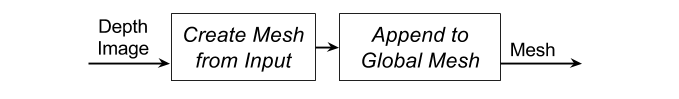
\includegraphics[width=.9\textwidth]{figures/diagram_general_pipeline_blackbox.png}
  \caption{Current methods}
  \label{fig:pipeline_cs}
\end{subfigure}
\begin{subfigure}[b]{\textwidth}
  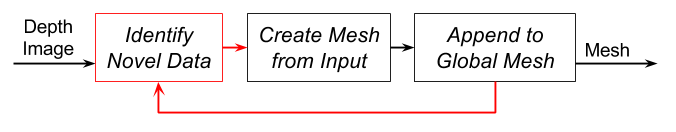
\includegraphics[width=.9\textwidth]{figures/diagram_general_pipeline_mabdi.png}
  \caption{MABDI}
  \label{fig:pipeline_mabdi}
\end{subfigure}
\caption{Algorithmic structure of current methods (a) and MABDI
(b). Contribution of MABDI to the state-of-the-art shown in red}
\label{fig:pipeline}
\end{figure}
